\section{Technický literárny prehľad}
DT predstavuje koncept virtuálnej repliky fyzického objektu alebo systému, ktorá je schopná v reálnom čase odrážať jeho aktuálny stav prostredníctvom obojsmernej výmeny dát (pozri Obr. \ref{fig:PLM}) \cite{DT:OriginToFuture}. Na rozdiel od tradičných modelov alebo simulácií je DT charakteristické dynamickým aktualizovaním svojho správania na základe dát zo sledovaného objektu \cite{systematicReview}. Tento koncept nachádza uplatnenie naprieč viacerými odvetviami vrátane výroby, zdravotníctva, dopravy či energetiky \cite{5gandbeyond}.\\

\begin{figure}[H]
    \centering
    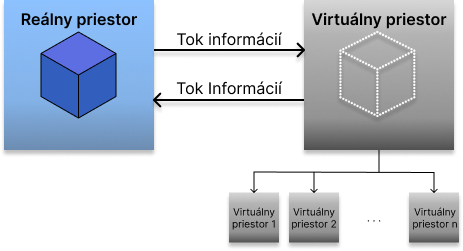
\includegraphics[width=0.8\linewidth]{assets/images/Grieves_PLM_model.png}
    \caption[Model zrkadlených priestorov]{Model zrkadlených priestorov (Mirrored Spaces Model) tak, ako ho vo svojej práci navrhol Grieves \cite{Grieves}. Tento model sa skladá z troch komponentov - reálny priestor (Real Space), virtuálny priestor (Virtual space) a spájací mechanizmus (Linking Mechanism) \cite{DT:OriginToFuture}, ktorý prúdi automatizovane oboma smermi medzi týmito priestormi. Virtuálny priestor vytvára digitálnu reprezentáciu reálnych objektov a podporuje viacero virtuálnych systémov na analýzu, simuláciu alebo predikciu správania fyzických objektov.}
    \label{fig:PLM}
\end{figure}

Vo  svojom výskume Enders a Hoßbachová \cite{DimensionOfDTAplication} identifikovali sektory, kde je používanie DT najrozšírenejšie. Patria sem výroba \cite{manuf}, letecký priemysel \cite{aircraft}, energetika \cite{energy}, automobilový priemysel \cite{automotive}, námorníctvo \cite{marine}, petrochemický priemysel \cite{oil}, poľnohospodárstvo \cite{agriculture}, zdravotníctvo \cite{health}, verejný sektor \cite{education} a ťažba \cite{mining}.

Taktiež identifikovali tri hlavné využitia DT v týchto oblastiach \cite{AplicationsOfDT}: ovládanie, simulovanie a monitorovanie. To však nepokrýva všetky možnosti a spôsoby využitia. DT dnes nájde uplatnenie aj pri dizajnovaní, validácii, predchádzaní chýb, trénovaní a optimalizácii.

Vývoj DT je podporený množstvom softvérových nástrojov líšiacich sa funkcionalitou a cenou. ANSYS Twin Builder je zameraný na presné fyzikálne modelovanie procesov (mechanika, elektromagnetizmus) a je vhodný pre tvorbu inžinierskych DT, pričom patrí medzi najnákladnejšie riešenia \cite{ansys_twin_builder}. Siemens MindSphere ponúka cloudovú platformu na správu dát a monitoring zariadení v priemyselných aplikáciách, s cenou závislou od rozsahu nasadenia \cite{siemens_mindsphere}. MATLAB a Simulink ponúkajú flexibilnú platformu pre tvorbu DT s dôrazom na simuláciu dynamických systémov, modelovanie riadiacich algoritmov a predikciu správania \cite{mathworks_digital_twin}.
Alternatívou bez licenčných nákladov je vlastná implementácia DT prostredí, kde je možné vytvoriť simulované kópie vybraných častí systému. Napríklad v oblasti 5G možno pomocou Open5GS a UERANSIM zostaviť základné virtuálne repliky siete, ktoré v kombinácii s vhodne naprogramovanými skriptami umožňujú budovanie DT.

Ak sa chceme pozrieť na reálne aplikácie DT, Huawei implementoval DT na monitorovanie výrobných liniek \cite{huawei2020}, zatiaľ čo mestá ako Bristol \cite{Bristol} či Singapur \cite{singapur} používajú DT na efektívne riadenie inteligentných mestských systémov. V týchto scenároch DT umožňuje predikciu zlyhaní, optimalizáciu zdrojov a minimalizáciu prestojov. 

V oblasti telekomunikácií umožňuje DT monitorovanie siete v reálnom čase, predikciu bezpečnostných incidentov a optimalizáciu konfigurácie bez zásahu do produkčnej infraštruktúry. Príkladom sú práce, ktoré implementovali DT do experimentálnych 5G jadier s cieľom analyzovať sieťové toky, detegovať anomálie a klasifikovať typ prevádzky pomocou strojového učenia \cite{DTof5G}.

Významnú úlohu tu zohráva výber príznakov, ktorý umožňuje redukovať výpočtovú náročnosť klasifikácie a zároveň zvyšuje robustnosť modelov v prostredí s vysokým objemom dát. Rôzne štúdie ukazujú, že výber príznakov výrazne ovplyvňuje výkon modelov najmä v prípade detekcie útokov distribuovaného odmietnutia služby (DoS) alebo neštandardného správania zariadení internetu vecí (IoT) v 5G jadre \cite{EffectiveFS}. Použité techniky zahŕňajú metódy ako Random Forest, k-najbližších susedov, rekurzívne odstraňovanie príznakov, permutačnú dôležitosť (PI) a ich kombinácie.

Z prehľadu literatúry vyplýva, že realistická simulácia sieťového správania a efektívna klasifikácia v reálnom čase si vyžadujú prepojenie viacerých nástrojov a metodík. Nasledujúca kapitola predstavuje konkrétny návrh a implementáciu DT systému, ktorý tieto poznatky aplikuje v kontexte 5G siete.
